\documentclass[]{article}
\usepackage{lmodern}
\usepackage{amssymb,amsmath}
\usepackage{ifxetex,ifluatex}
\usepackage{fixltx2e} % provides \textsubscript
\ifnum 0\ifxetex 1\fi\ifluatex 1\fi=0 % if pdftex
  \usepackage[T1]{fontenc}
  \usepackage[utf8]{inputenc}
\else % if luatex or xelatex
  \ifxetex
    \usepackage{mathspec}
  \else
    \usepackage{fontspec}
  \fi
  \defaultfontfeatures{Ligatures=TeX,Scale=MatchLowercase}
\fi
% use upquote if available, for straight quotes in verbatim environments
\IfFileExists{upquote.sty}{\usepackage{upquote}}{}
% use microtype if available
\IfFileExists{microtype.sty}{%
\usepackage{microtype}
\UseMicrotypeSet[protrusion]{basicmath} % disable protrusion for tt fonts
}{}
\usepackage[margin=1in]{geometry}
\usepackage{hyperref}
\hypersetup{unicode=true,
            pdftitle={STATS 205: Homework Assignment 3},
            pdfauthor={Brian Liu},
            pdfborder={0 0 0},
            breaklinks=true}
\urlstyle{same}  % don't use monospace font for urls
\usepackage{color}
\usepackage{fancyvrb}
\newcommand{\VerbBar}{|}
\newcommand{\VERB}{\Verb[commandchars=\\\{\}]}
\DefineVerbatimEnvironment{Highlighting}{Verbatim}{commandchars=\\\{\}}
% Add ',fontsize=\small' for more characters per line
\usepackage{framed}
\definecolor{shadecolor}{RGB}{248,248,248}
\newenvironment{Shaded}{\begin{snugshade}}{\end{snugshade}}
\newcommand{\AlertTok}[1]{\textcolor[rgb]{0.94,0.16,0.16}{#1}}
\newcommand{\AnnotationTok}[1]{\textcolor[rgb]{0.56,0.35,0.01}{\textbf{\textit{#1}}}}
\newcommand{\AttributeTok}[1]{\textcolor[rgb]{0.77,0.63,0.00}{#1}}
\newcommand{\BaseNTok}[1]{\textcolor[rgb]{0.00,0.00,0.81}{#1}}
\newcommand{\BuiltInTok}[1]{#1}
\newcommand{\CharTok}[1]{\textcolor[rgb]{0.31,0.60,0.02}{#1}}
\newcommand{\CommentTok}[1]{\textcolor[rgb]{0.56,0.35,0.01}{\textit{#1}}}
\newcommand{\CommentVarTok}[1]{\textcolor[rgb]{0.56,0.35,0.01}{\textbf{\textit{#1}}}}
\newcommand{\ConstantTok}[1]{\textcolor[rgb]{0.00,0.00,0.00}{#1}}
\newcommand{\ControlFlowTok}[1]{\textcolor[rgb]{0.13,0.29,0.53}{\textbf{#1}}}
\newcommand{\DataTypeTok}[1]{\textcolor[rgb]{0.13,0.29,0.53}{#1}}
\newcommand{\DecValTok}[1]{\textcolor[rgb]{0.00,0.00,0.81}{#1}}
\newcommand{\DocumentationTok}[1]{\textcolor[rgb]{0.56,0.35,0.01}{\textbf{\textit{#1}}}}
\newcommand{\ErrorTok}[1]{\textcolor[rgb]{0.64,0.00,0.00}{\textbf{#1}}}
\newcommand{\ExtensionTok}[1]{#1}
\newcommand{\FloatTok}[1]{\textcolor[rgb]{0.00,0.00,0.81}{#1}}
\newcommand{\FunctionTok}[1]{\textcolor[rgb]{0.00,0.00,0.00}{#1}}
\newcommand{\ImportTok}[1]{#1}
\newcommand{\InformationTok}[1]{\textcolor[rgb]{0.56,0.35,0.01}{\textbf{\textit{#1}}}}
\newcommand{\KeywordTok}[1]{\textcolor[rgb]{0.13,0.29,0.53}{\textbf{#1}}}
\newcommand{\NormalTok}[1]{#1}
\newcommand{\OperatorTok}[1]{\textcolor[rgb]{0.81,0.36,0.00}{\textbf{#1}}}
\newcommand{\OtherTok}[1]{\textcolor[rgb]{0.56,0.35,0.01}{#1}}
\newcommand{\PreprocessorTok}[1]{\textcolor[rgb]{0.56,0.35,0.01}{\textit{#1}}}
\newcommand{\RegionMarkerTok}[1]{#1}
\newcommand{\SpecialCharTok}[1]{\textcolor[rgb]{0.00,0.00,0.00}{#1}}
\newcommand{\SpecialStringTok}[1]{\textcolor[rgb]{0.31,0.60,0.02}{#1}}
\newcommand{\StringTok}[1]{\textcolor[rgb]{0.31,0.60,0.02}{#1}}
\newcommand{\VariableTok}[1]{\textcolor[rgb]{0.00,0.00,0.00}{#1}}
\newcommand{\VerbatimStringTok}[1]{\textcolor[rgb]{0.31,0.60,0.02}{#1}}
\newcommand{\WarningTok}[1]{\textcolor[rgb]{0.56,0.35,0.01}{\textbf{\textit{#1}}}}
\usepackage{graphicx,grffile}
\makeatletter
\def\maxwidth{\ifdim\Gin@nat@width>\linewidth\linewidth\else\Gin@nat@width\fi}
\def\maxheight{\ifdim\Gin@nat@height>\textheight\textheight\else\Gin@nat@height\fi}
\makeatother
% Scale images if necessary, so that they will not overflow the page
% margins by default, and it is still possible to overwrite the defaults
% using explicit options in \includegraphics[width, height, ...]{}
\setkeys{Gin}{width=\maxwidth,height=\maxheight,keepaspectratio}
\IfFileExists{parskip.sty}{%
\usepackage{parskip}
}{% else
\setlength{\parindent}{0pt}
\setlength{\parskip}{6pt plus 2pt minus 1pt}
}
\setlength{\emergencystretch}{3em}  % prevent overfull lines
\providecommand{\tightlist}{%
  \setlength{\itemsep}{0pt}\setlength{\parskip}{0pt}}
\setcounter{secnumdepth}{0}
% Redefines (sub)paragraphs to behave more like sections
\ifx\paragraph\undefined\else
\let\oldparagraph\paragraph
\renewcommand{\paragraph}[1]{\oldparagraph{#1}\mbox{}}
\fi
\ifx\subparagraph\undefined\else
\let\oldsubparagraph\subparagraph
\renewcommand{\subparagraph}[1]{\oldsubparagraph{#1}\mbox{}}
\fi

%%% Use protect on footnotes to avoid problems with footnotes in titles
\let\rmarkdownfootnote\footnote%
\def\footnote{\protect\rmarkdownfootnote}

%%% Change title format to be more compact
\usepackage{titling}

% Create subtitle command for use in maketitle
\providecommand{\subtitle}[1]{
  \posttitle{
    \begin{center}\large#1\end{center}
    }
}

\setlength{\droptitle}{-2em}

  \title{STATS 205: Homework Assignment 3}
    \pretitle{\vspace{\droptitle}\centering\huge}
  \posttitle{\par}
    \author{Brian Liu}
    \preauthor{\centering\large\emph}
  \postauthor{\par}
      \predate{\centering\large\emph}
  \postdate{\par}
    \date{4/26/2019}


\begin{document}
\maketitle

\hypertarget{solution-to-problem-1}{%
\subsection{Solution to Problem 1}\label{solution-to-problem-1}}

\hypertarget{i}{%
\subsubsection{(i)}\label{i}}

\begin{Shaded}
\begin{Highlighting}[]
\KeywordTok{library}\NormalTok{(bootstrap); }\KeywordTok{data}\NormalTok{(law)}
\KeywordTok{t}\NormalTok{(law)}
\end{Highlighting}
\end{Shaded}

\begin{verbatim}
##           1     2      3      4      5      6   7      8      9     10
## LSAT 576.00 635.0 558.00 578.00 666.00 580.00 555 661.00 651.00 605.00
## GPA    3.39   3.3   2.81   3.03   3.44   3.07   3   3.43   3.36   3.13
##          11     12     13     14     15
## LSAT 653.00 575.00 545.00 572.00 594.00
## GPA    3.12   2.74   2.76   2.88   2.96
\end{verbatim}

\begin{Shaded}
\begin{Highlighting}[]
\NormalTok{theta.hat =}\StringTok{ }\KeywordTok{cor}\NormalTok{(law}\OperatorTok{$}\NormalTok{LSAT, law}\OperatorTok{$}\NormalTok{GPA); theta.hat}
\end{Highlighting}
\end{Shaded}

\begin{verbatim}
## [1] 0.7763745
\end{verbatim}

\begin{Shaded}
\begin{Highlighting}[]
\KeywordTok{library}\NormalTok{(partitions)}
\NormalTok{n =}\StringTok{ }\DecValTok{15}
\NormalTok{allCompositions =}\StringTok{ }\KeywordTok{compositions}\NormalTok{(n, n);allCompositions[,}\DecValTok{1}\OperatorTok{:}\DecValTok{5}\NormalTok{]}
\end{Highlighting}
\end{Shaded}

\begin{verbatim}
##       [,1] [,2] [,3] [,4] [,5]
##  [1,]   15   14   13   12   11
##  [2,]    0    1    2    3    4
##  [3,]    0    0    0    0    0
##  [4,]    0    0    0    0    0
##  [5,]    0    0    0    0    0
##  [6,]    0    0    0    0    0
##  [7,]    0    0    0    0    0
##  [8,]    0    0    0    0    0
##  [9,]    0    0    0    0    0
## [10,]    0    0    0    0    0
## [11,]    0    0    0    0    0
## [12,]    0    0    0    0    0
## [13,]    0    0    0    0    0
## [14,]    0    0    0    0    0
## [15,]    0    0    0    0    0
\end{verbatim}

\begin{Shaded}
\begin{Highlighting}[]
\NormalTok{allCompositions.sub =}\StringTok{ }\NormalTok{allCompositions[, }\KeywordTok{sample}\NormalTok{(}\DecValTok{1}\OperatorTok{:}\KeywordTok{dim}\NormalTok{(allCompositions)[}\DecValTok{2}\NormalTok{], }\DataTypeTok{size=}\DecValTok{10000}\NormalTok{, }\DataTypeTok{replace=}\OtherTok{FALSE}\NormalTok{)]}

\NormalTok{draw.bootstrap.samples =}\StringTok{ }\ControlFlowTok{function}\NormalTok{(df)\{}
\NormalTok{  n =}\StringTok{ }\KeywordTok{dim}\NormalTok{(df)[}\DecValTok{1}\NormalTok{]}
\NormalTok{  ind =}\StringTok{ }\KeywordTok{sample}\NormalTok{(n, }\DataTypeTok{replace =} \OtherTok{TRUE}\NormalTok{)}
\NormalTok{  cor.bootstrap.replicate =}\StringTok{ }\KeywordTok{cor}\NormalTok{(df[ind, }\StringTok{"LSAT"}\NormalTok{], df[ind, }\StringTok{"GPA"}\NormalTok{])}
  \KeywordTok{return}\NormalTok{(cor.bootstrap.replicate)}
\NormalTok{\}}
\NormalTok{R =}\StringTok{ }\DecValTok{10000}
\NormalTok{theta.hat.star =}\StringTok{ }\KeywordTok{replicate}\NormalTok{(R, }\KeywordTok{draw.bootstrap.samples}\NormalTok{(law))}
\CommentTok{# make a ggplot}
\KeywordTok{library}\NormalTok{(ggplot2)}
\end{Highlighting}
\end{Shaded}

\begin{verbatim}
## Registered S3 methods overwritten by 'ggplot2':
##   method         from 
##   [.quosures     rlang
##   c.quosures     rlang
##   print.quosures rlang
\end{verbatim}

\begin{Shaded}
\begin{Highlighting}[]
\NormalTok{theta.hat.star.df =}\StringTok{ }\KeywordTok{data.frame}\NormalTok{(}\DataTypeTok{theta.hat.star =}\NormalTok{ theta.hat.star)}
\KeywordTok{ggplot}\NormalTok{(theta.hat.star.df) }\OperatorTok{+}
\StringTok{  }\KeywordTok{geom_density}\NormalTok{(}\KeywordTok{aes}\NormalTok{(}\DataTypeTok{x =}\NormalTok{ theta.hat.star, }\DataTypeTok{y =}\NormalTok{ ..scaled..),}
    \DataTypeTok{fill =} \StringTok{"lightblue"}\NormalTok{) }\OperatorTok{+}
\StringTok{  }\KeywordTok{geom_hline}\NormalTok{(}\DataTypeTok{yintercept=}\DecValTok{0}\NormalTok{, }\DataTypeTok{colour=}\StringTok{"white"}\NormalTok{, }\DataTypeTok{size=}\DecValTok{1}\NormalTok{) }\OperatorTok{+}
\StringTok{  }\KeywordTok{theme_bw}\NormalTok{() }\OperatorTok{+}
\StringTok{  }\KeywordTok{ylab}\NormalTok{(}\StringTok{"density"}\NormalTok{) }\OperatorTok{+}
\StringTok{  }\KeywordTok{xlab}\NormalTok{(}\KeywordTok{bquote}\NormalTok{(}\KeywordTok{hat}\NormalTok{(theta))) }\OperatorTok{+}
\StringTok{  }\KeywordTok{geom_vline}\NormalTok{(}\DataTypeTok{xintercept =}\NormalTok{ theta.hat, }\DataTypeTok{col =} \StringTok{"red"}\NormalTok{)}\OperatorTok{+}
\StringTok{  }\KeywordTok{scale_y_continuous}\NormalTok{(}\DataTypeTok{expand =} \KeywordTok{c}\NormalTok{(}\DecValTok{0}\NormalTok{,}\DecValTok{0}\NormalTok{))}
\end{Highlighting}
\end{Shaded}

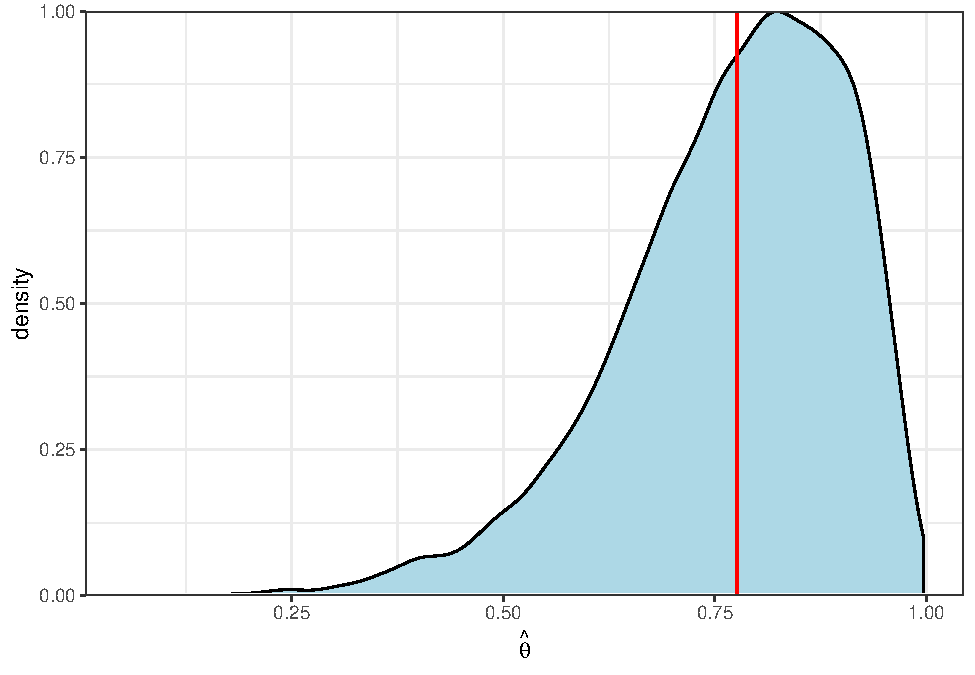
\includegraphics{homework_3_files/figure-latex/unnamed-chunk-1-1.pdf}

\hypertarget{ii}{%
\subsubsection{(ii)}\label{ii}}

\begin{Shaded}
\begin{Highlighting}[]
\KeywordTok{sd}\NormalTok{(theta.hat.star)}
\end{Highlighting}
\end{Shaded}

\begin{verbatim}
## [1] 0.1339632
\end{verbatim}

\hypertarget{solution-to-problem-2}{%
\subsection{Solution to Problem 2}\label{solution-to-problem-2}}

\hypertarget{i-1}{%
\subsubsection{(i)}\label{i-1}}

\begin{verbatim}
67 runs resulting in swallowing attempts
58 successful
9 failed

H_0 : p = 0.6
H_A : p > 0.6

\end{verbatim}

\begin{Shaded}
\begin{Highlighting}[]
\NormalTok{n =}\StringTok{ }\DecValTok{67}
\NormalTok{successes =}\StringTok{ }\DecValTok{58}
\NormalTok{pbar =}\StringTok{ }\NormalTok{successes }\OperatorTok{/}\StringTok{ }\NormalTok{n; pbar}
\end{Highlighting}
\end{Shaded}

\begin{verbatim}
## [1] 0.8656716
\end{verbatim}

\begin{Shaded}
\begin{Highlighting}[]
\NormalTok{p0 =}\StringTok{ }\FloatTok{0.6}\NormalTok{; nsim =}\StringTok{ }\DecValTok{10000}
\NormalTok{B =}\StringTok{ }\KeywordTok{rbinom}\NormalTok{(nsim, }\DataTypeTok{size =}\NormalTok{ n, }\DataTypeTok{prob =}\NormalTok{ p0)}
\KeywordTok{hist}\NormalTok{(B, }\DataTypeTok{breaks =} \DecValTok{30}\NormalTok{)}
\end{Highlighting}
\end{Shaded}

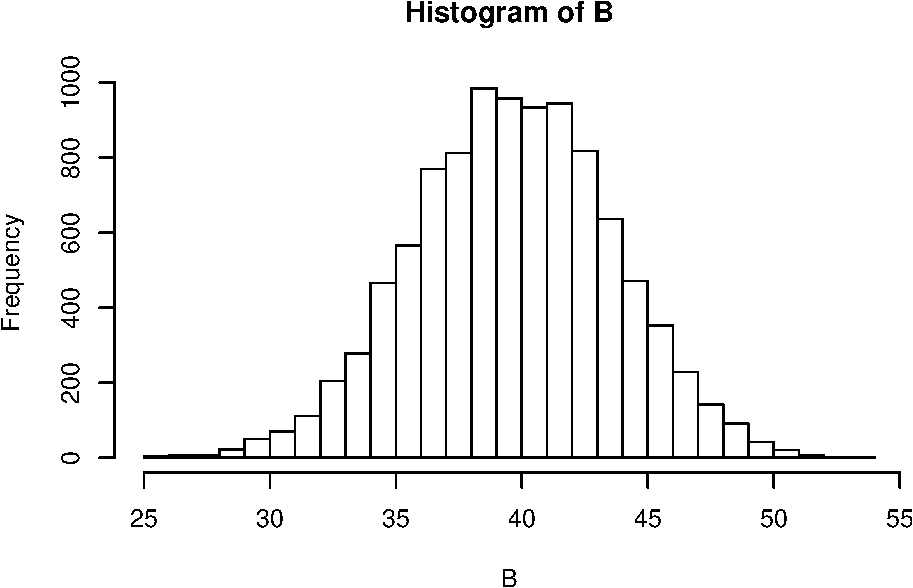
\includegraphics{homework_3_files/figure-latex/unnamed-chunk-3-1.pdf}

Test statistic \(Z\):

\[
    Z_0 = \frac{B - 67(0.6)}{(67(0.6)(0.4))^{\frac{1}{2}}}
\]

\begin{Shaded}
\begin{Highlighting}[]
\KeywordTok{qnorm}\NormalTok{((}\DecValTok{1}\FloatTok{-0.05}\NormalTok{), }\DataTypeTok{mean =} \DecValTok{0}\NormalTok{, }\DataTypeTok{sd =} \DecValTok{1}\NormalTok{)}
\end{Highlighting}
\end{Shaded}

\begin{verbatim}
## [1] 1.644854
\end{verbatim}

Rejection region: \(Z \geq z_{0.05} = 1.645\)

Observed test statistic \(Z_o\):

\[
    Z_o = \frac{58 - 67(0.6)}{(67(0.6)(0.4))^{\frac{1}{2}}} = 4.44
\]

\begin{Shaded}
\begin{Highlighting}[]
\NormalTok{numerator =}\StringTok{ }\NormalTok{successes }\OperatorTok{-}\StringTok{ }\NormalTok{(n }\OperatorTok{*}\StringTok{ }\NormalTok{p0)}
\NormalTok{denominator =}\StringTok{ }\KeywordTok{sqrt}\NormalTok{(n }\OperatorTok{*}\StringTok{ }\NormalTok{p0 }\OperatorTok{*}\StringTok{ }\NormalTok{(}\FloatTok{1.0} \OperatorTok{-}\StringTok{ }\NormalTok{p0))}
\NormalTok{Z.obs =}\StringTok{ }\NormalTok{numerator }\OperatorTok{/}\StringTok{ }\NormalTok{denominator; Z.obs}
\end{Highlighting}
\end{Shaded}

\begin{verbatim}
## [1] 4.438917
\end{verbatim}

The large sample approximation value \(Z_o = 2.5 > 1.645\) and thus we
reject \(H_0 : p = 0.6\) in favor of \(p > 0.6\) at the approximate
\(\alpha = 0.05\) level. Thus there is evidence that the success rate of
swallowing attempts is greater than \(0.6\).

\hypertarget{ii-1}{%
\subsubsection{(ii)}\label{ii-1}}

Power is the probability of rejecting \(H_0\) when \(H_A\) is true. We
found that test reject \(H_0\) is \(Z \geq z_{0.05} = 1.645\).
Therefore, if \(p = 0.7\),

\[
    Z_o = \frac{58 - 67(0.6)}{(67(0.6)(0.4))^{\frac{1}{2}}} = 4.44
\]

is no longer standard normal.

We have

\[
    Z_{o7} = \frac{58 - 67(0.7)}{(67(0.7)(0.3))^{\frac{1}{2}}} = 2.96
\]

\begin{Shaded}
\begin{Highlighting}[]
\NormalTok{p1 =}\StringTok{ }\FloatTok{0.7}
\NormalTok{numerator =}\StringTok{ }\NormalTok{successes }\OperatorTok{-}\StringTok{ }\NormalTok{(n }\OperatorTok{*}\StringTok{ }\NormalTok{p1)}
\NormalTok{denominator =}\StringTok{ }\KeywordTok{sqrt}\NormalTok{(n }\OperatorTok{*}\StringTok{ }\NormalTok{p1 }\OperatorTok{*}\StringTok{ }\NormalTok{(}\FloatTok{1.0} \OperatorTok{-}\StringTok{ }\NormalTok{p1))}
\NormalTok{Z.obs.seven =}\StringTok{ }\NormalTok{numerator }\OperatorTok{/}\StringTok{ }\NormalTok{denominator; Z.obs.seven}
\end{Highlighting}
\end{Shaded}

\begin{verbatim}
## [1] 2.959211
\end{verbatim}

\[
    Power = P(Z \geq 1.645 | p = 0.7)
\]

\[
    = P_{p = 0.7}\bigg(\frac{B - 67(0.6)}{(67(0.6)(0.4))^{\frac{1}{2}}} \geq 1.645\bigg)
\]

\[
    = P_{p = 0.7}(B \geq 1.645(67(0.6)(0.4))^{\frac{1}{2}} + 67(0.6))
\]

\[
    = P_{p=0.7}\bigg(\frac{B - 67(0.7)}{(67(0.7)(0.3))^{\frac{1}{2}}} \geq \frac{1.645(67(0.6)(0.4))^{\frac{1}{2}} + 67(0.6) - 67(0.7)}{(67(0.7)(0.3))^{\frac{1}{2}}}\bigg)
\]

\begin{Shaded}
\begin{Highlighting}[]
\NormalTok{triple_product =}\StringTok{ }\NormalTok{n }\OperatorTok{*}\StringTok{ }\NormalTok{p0 }\OperatorTok{*}\StringTok{ }\NormalTok{(}\FloatTok{1.0} \OperatorTok{-}\StringTok{ }\NormalTok{p0)}
\NormalTok{first_term =}\StringTok{ }\FloatTok{1.645} \OperatorTok{*}\StringTok{ }\KeywordTok{sqrt}\NormalTok{(triple_product)}
\NormalTok{second_term =}\StringTok{ }\NormalTok{n }\OperatorTok{*}\StringTok{ }\NormalTok{p0}
\NormalTok{third_term =}\StringTok{ }\NormalTok{n }\OperatorTok{*}\StringTok{ }\NormalTok{p1}
\NormalTok{bottom_term =}\StringTok{ }\NormalTok{n }\OperatorTok{*}\StringTok{ }\NormalTok{p1 }\OperatorTok{*}\StringTok{ }\NormalTok{(}\FloatTok{1.0} \OperatorTok{-}\StringTok{ }\NormalTok{p1)}
\NormalTok{p7_numerator =}\StringTok{ }\NormalTok{first_term }\OperatorTok{+}\StringTok{ }\NormalTok{second_term }\OperatorTok{-}\StringTok{ }\NormalTok{third_term}
\NormalTok{p7_denominator =}\StringTok{ }\KeywordTok{sqrt}\NormalTok{(bottom_term)}
\NormalTok{Pp_}\DecValTok{7}\NormalTok{_zvalue =}\StringTok{ }\NormalTok{p7_numerator }\OperatorTok{/}\StringTok{ }\NormalTok{p7_denominator; Pp_}\DecValTok{7}\NormalTok{_zvalue}
\end{Highlighting}
\end{Shaded}

\begin{verbatim}
## [1] -0.02761144
\end{verbatim}

\[
    P(Z^* \geq -0.0276) = 0.4890
\]

\begin{Shaded}
\begin{Highlighting}[]
\CommentTok{# pvalue = pnorm(-abs(Pp_7_zvalue)); pvalue}
\NormalTok{pvalue =}\StringTok{ }\KeywordTok{pnorm}\NormalTok{(Pp_}\DecValTok{7}\NormalTok{_zvalue); pvalue}
\end{Highlighting}
\end{Shaded}

\begin{verbatim}
## [1] 0.488986
\end{verbatim}

If \(p = 0.8\),

\[
    Power = P(Z \geq 1.645 | p = 0.8)
\]

\[
    = P_{p=0.8}\bigg(\frac{B - 67(0.8)}{(67(0.8)(0.2))^{\frac{1}{2}}} \geq \frac{1.645(67(0.6)(0.4))^{\frac{1}{2}} + 67(0.6) - 67(0.8)}{(67(0.8)(0.2))^{\frac{1}{2}}}\bigg)
\]

\begin{Shaded}
\begin{Highlighting}[]
\NormalTok{p2 =}\StringTok{ }\FloatTok{0.8}
\NormalTok{triple_product =}\StringTok{ }\NormalTok{n }\OperatorTok{*}\StringTok{ }\NormalTok{p0 }\OperatorTok{*}\StringTok{ }\NormalTok{(}\FloatTok{1.0} \OperatorTok{-}\StringTok{ }\NormalTok{p0)}
\NormalTok{first_term =}\StringTok{ }\FloatTok{1.645} \OperatorTok{*}\StringTok{ }\KeywordTok{sqrt}\NormalTok{(triple_product)}
\NormalTok{second_term =}\StringTok{ }\NormalTok{n }\OperatorTok{*}\StringTok{ }\NormalTok{p0}
\NormalTok{third_term =}\StringTok{ }\NormalTok{n }\OperatorTok{*}\StringTok{ }\NormalTok{p2}
\NormalTok{bottom_term =}\StringTok{ }\NormalTok{n }\OperatorTok{*}\StringTok{ }\NormalTok{p2 }\OperatorTok{*}\StringTok{ }\NormalTok{(}\FloatTok{1.0} \OperatorTok{-}\StringTok{ }\NormalTok{p2)}
\NormalTok{p8_numerator =}\StringTok{ }\NormalTok{first_term }\OperatorTok{+}\StringTok{ }\NormalTok{second_term }\OperatorTok{-}\StringTok{ }\NormalTok{third_term}
\NormalTok{p8_denominator =}\StringTok{ }\KeywordTok{sqrt}\NormalTok{(bottom_term)}
\NormalTok{Pp_}\DecValTok{8}\NormalTok{_zvalue =}\StringTok{ }\NormalTok{p8_numerator }\OperatorTok{/}\StringTok{ }\NormalTok{p8_denominator; Pp_}\DecValTok{8}\NormalTok{_zvalue}
\end{Highlighting}
\end{Shaded}

\begin{verbatim}
## [1] -2.077971
\end{verbatim}

\[
    P(Z^* \geq -2.078) = 0.01886
\]

\begin{Shaded}
\begin{Highlighting}[]
\CommentTok{# pvalue = pnorm(-abs(Pp_7_zvalue)); pvalue}
\NormalTok{pvalue =}\StringTok{ }\KeywordTok{pnorm}\NormalTok{(Pp_}\DecValTok{8}\NormalTok{_zvalue); pvalue}
\end{Highlighting}
\end{Shaded}

\begin{verbatim}
## [1] 0.01885601
\end{verbatim}

\hypertarget{solution-to-problem-3}{%
\subsection{Solution to Problem 3}\label{solution-to-problem-3}}

\begin{Shaded}
\begin{Highlighting}[]
\KeywordTok{library}\NormalTok{(binom)}
\KeywordTok{binom.confint}\NormalTok{(}\DataTypeTok{x=}\DecValTok{56}\NormalTok{, }\DataTypeTok{n=}\DecValTok{65}\NormalTok{, }\DataTypeTok{conf.level=}\NormalTok{.}\DecValTok{95}\NormalTok{, }\DataTypeTok{methods =} \StringTok{"asymptotic"}\NormalTok{)}
\end{Highlighting}
\end{Shaded}

\begin{verbatim}
##       method  x  n      mean     lower     upper
## 1 asymptotic 56 65 0.8615385 0.7775744 0.9455025
\end{verbatim}

\$\hat{p} = (0.7776, 0.9455)

\begin{Shaded}
\begin{Highlighting}[]
\KeywordTok{library}\NormalTok{(beepr)}
\KeywordTok{beep}\NormalTok{()}
\end{Highlighting}
\end{Shaded}


\end{document}
